
\chapter{Literature Review} 

\label{Chapter2} 

\lhead{Chapter 2. \emph{State of the Art}} 

\section{Introduction}

This section introduces fields of study under investigation in this project, Machine Learning and Defeasible Reasoning. The existing literature on both areas is reviewed in order to provide the reader with an understanding of the context in which the research occurs. As the project is fundamentally a comparison between the two fields this literature review also gathers results and conclusions from other work that will help to inform this comparison. This material will be used to support the arguments made for both approaches and will also inform the design of an experiment evaluating the approaches. At a high level this project examines two differing approaches to artificial intelligence, knowledge-base approaches and learning based approaches (machine learning).

\begin{figure}[!h]
\centering
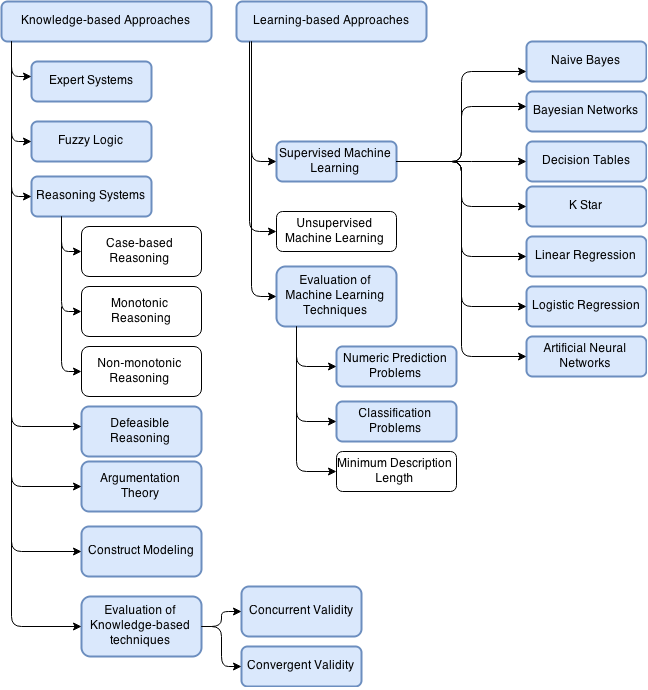
\includegraphics[width=\linewidth]{Chapter2}
\caption{Chapter Overview}
\label{fig:chapter_overview}
\end{figure}

\cite{mitchell2006discipline} defines machine learning as a field of computer science that attempts to solve the question:

``How can we build computer systems that automatically improve with experience, and what are the fundamental laws that govern all learning processes?''

On a practical level it is an area of study that concerns itself with the design of techniques and algorithms that run uniquely on different data to achieve some aim without being explicitly programmed. A machine learning program initial takes a data as input which it learns from; this learning is then used on future inputs to make a prediction or to provide some understanding. Mitchell outlines that while there had been no successful commercial applications of machine learning as late as 1985, it has since been successfully applied in diverse fields such as speech recognition, computer vision, bio-surveillance, robot control and accelerating empirical sciences. Indeed in the last several years some of the biggest names in technology such as IBM, Google, Microsoft and Baidu have been making great strides in the development of advanced machine learning techniques and reaping the rewards.

Knowledge-base approaches differ from learning approaches in that instead of learning from labeled data, the software makes decisions based on `knowledge'. The software is not explicitly programmed to perform operations on the data; a knowledge based approach takes a knowledge base and uses it's contents to make inferences based on data. The most common example of a knowledge based approach is in expert systems where the knowledge base is that of an expert. The knowledge used in KB systems can have many forms such as natural language text, mathematical functions and raw data. Some knowledge based systems may infact learn from previous experience, for example, in CASE-based reasoning in which solutions for new cases may be added to the repository of cases used for inference.



















\section{Knowledge-Based Approaches}

\cite{akerkar2010knowledge} describe knowledge based systems as distinct from traditional information systems as they have an understanding of the data that they process. This understanding comes from a knowledge base made up of data, information and knowledge. Knowledge-base systems tend to be made up of a knowledge base and an inference engine, a program that can infer outcomes from the knowledge base given some input. Knowledge-base systems include expert systems and CASE-based reasoning systems. 

Key issues in knowledge based systems include the acquisition of knowledge, the representation of knowledge and reasoning about that knowledge.

In order to develop expert systems a knowledge engineer must gather domain expertise. This knowledge is elicited in a number of ways. Typically the knowledge engineer is not an expert in the domain and will gather the knowledge from books, journals and other sources. It may be more efficient for the knowledge engineer to elicit a knowledge base directly from an expert by interviewing them. Although this approach is preferable it is not always possible as the expert is busy with other work and unavailable for the long periods of time required to build a knowledge base. According to \cite{sagheb2009conceptual} in the early 1990's the most popular means of eliciting knowledge from an expert was the structured interview; other techniques include unstructured interviews, documentation and case study analysis, simulations and observation. 

\cite{davis1993knowledge} identifies five fundamental roles of knowledge representation. A knowledge representation is a surrogate; an imperfect stand in for something in the real world. Since it is imperfect, inferences made from it won't always be correct. The author discusses knowledge representation as an `ontological commitment'; by choosing one knowledge representation strategy over another we become bound to it and the ontology will have an influence on how reality is interpreted. A knowledge representation is a `fragmentary theory of intelligent reasoning'; the choice of knowledge representation influences what can be infered from it and is opinionated with regards to what it means to reason intelligently. A knowledge representation is a medium for efficient computation; it doesn't gather every nuance of reality, if it did the problems it is attempting to solve would be computationally intractable. Lastly the author explains that a KR is a medium of human expression; like programming languages, KRs are used for communicating not just with the system but with other knowledge engineers as well.

\cite{petrik2004knowledge} provides descriptions of a number of knowledge representation strategies employed in expert systems examples of which include semantic networks, frames, logic, bayes networks and influence diagrams. 

Rules are a form of KR in which the knowledge is encoded using if-then clauses activated with some heuristic function. Rules can be examined through the lens of the five roles propsed by \cite{davis1993knowledge}. As a surrogate rules are poor at modeling complex relationships. By choosing to use rules for KR in a system the ontology will be overly simplified. It's theory of reasoning is that everything can be represented as an action to take in a given situation. Thanks to fast Rete matching algorithms it is an effective medium for computation for simple problems. As a medium of human expresion it is desirable; as rules can be formulated in natural language, they are easy to understand and to create.

\subsection{Expert Systems}

\cite{todd1992introduction} describes an expert system as one in which an inference mechanism is applied to the knowledge of an expert. Expert systems typically are employed in decision support systems in which they may provide assistance in tasks such as diagnosis. Expert systems typically have to reason with imprecise and incomplete information and various means have been adopted to deal with this information in expert systems. \cite{kandel1991fuzzy} explains how two implementations CASNET and MYCIN handle these uncertainties; the later uses certainty factors while the former uses the most significant results of tests.

\cite{kandel1991fuzzy} goes on to describe how fuzzy logic like that proposed by \cite{zadeh1965fuzzy} has been utilsed in expert systems to deal with uncertainty. In a nutshell fuzzy sets attempt to define the membership of a set by quantifying it. Membership is defined using membership functions which take an instance as input and quantify it's membership as a real number in the range zero and one. If the output of the membership function is zero then the instance is not a member of the set; on the other hand if it is one then the input is a member of the set. The values in between zero and one define the degree to which the instance is a member of the set.

\section{Reasoning Systems}

Once knowledge has been acquired and represented it is reasoned about using an inference engine. Reasoning involves using some known knowledge to deduce logical consequences. \cite{singh2010comparative} provides a comparison between different inference engines. Jess utilises rule based inference to make inferences. Hoolet translates it's ontology to a collection of axioms which are reasoned about using first order logic. Pellet uses probabilistic means of inference. All of these different engines attempt to make inferences based on imperfect data. In the last 20 years or so interest has increased in using defeasible reasoning and argumentation theory to make these inferences in the absences of consistent data. AT provides a model of reasoning that is both intuitive and computable.

\subsection{Case-Based Reasoning}

According to \cite{leake2003case}, the knowledge base of a case-based reasoning system consists of knowledge obtained in the past from solving problems (previous cases). When the system encounters a new situation not accounted for by the knowledge base, cases that may be relevant and useful are brought up and adapted to solve the new problem. The resulting new solution is then saved to the knowledge base for future use. Through the process of solving new problems the system effectively learns. CBR has the advantage of not requiring new solutions to be generated when familiar problems are encountered. CBR has applications in tasks such as interpreting the law, informing design and diagnosis.

\subsection{Non-Monotonic Reasoning}

\cite{baroni1997full} explains that \textit{monotonic} reasoning can be defined as follows: Given three sets $A, B, C$, if $A \vdash B$ then also $\(A \cup C\) \vdash B$. Informally, monotonic reasoning can be thought of a reasoning in which the conclusions for an argument are embedded in the premises and are not retracted in the light of new evidence. The truth that results from one statement cannot be retracted as a result of new evidence in monotonic reasoning. Monotonic reasoning is unhelpful in deducing the truth and as a result researchers have formulated non-monotonic reasoning to better model human reasoning. In non-monotonic reasoning conclusions can be retracted in light of new evidence. In our day to day activities humans make assumptions based on past experience. If a person lives in a part of the world that often has sunny weather then they assume this to be true by default and generally behave as if it is going to be that way. If the weather forecast warns them of heavy rain they will retract their conclusion that today will be sunny and bring an umbrella. The logic of making assumptions is known as default logic. Default logic allows us to make assumptions with incomplete evidence based on what we believe to typically be the case. Non-monotonic reasoning allows us to override these defaults when presented with new information.

\section{Defeasible Reasoning}

Argumentation theory has it's roots in philosophy and is concerned with how issues are discussed and conclusions arrived at in the context of incomplete and conflicting evidence. The ability to deal with inconsistent information through reasoning is what has motivated it's use in AI. 

\cite{reiter1980logic} recognised the need to make assumptions when presented with incomplete evidence and to change these assumptions when presented with new evidence. Reiter recognised that classical logic is insufficient for dealing with these situations and proposed a logic for default reasoning. Default reasoning is a formalisation of what we believe to be true in the absence of other evidence that makes the case exceptional; what we believe to be true by default.

Default logic is a non-monotonic logic. Reiter describes first order logic as monotonic - conclusions drawn in the presence of information A remain valid in the presence of new information B. Non-monotonic reasoning provides a mechanism for revising old beliefs in the presence of new information. Default logic takes into account that conclusions drawn in the case of A may not be true in the case of B.

Take the example “Tweety is a bird, birds can fly, therefore Tweety can fly.” Tweety being able to fly is inferred by default since Tweety is a bird. If Tweety is a penguin, on the other hand, Tweety cannot fly. In first order logic we would still believe that Tweety can fly eventhough it is a penguin. Default logic allows us to revise our belief about what can fly. Our new belief can be that ``Birds fly, unless they are penguins''.

\cite{pollock1987defeasible} recognised that while non-monotonic logic in AI is similar to how humans reason, it was also falling short in it’s recognition of the complexities of reasoning. Pollock introduced the concept of defeasible reasoning, similar to nonmonotonic reasoning, to AI to better model these complexities. Reasoning can be said to be defeasible if the premises taken in isolation can infer a conclusion, but that this conclusion can be defeated when additional information is added. An important element of Pollock's defeasible reasoning is the idea of warrant; he defined a proposition as being warranted if it would be believed by an ideal reasoner. The conditions that determine whether an argument is warranted are made explicit by his work and include notions such as defeat relations between arguments.

\subsection{Argumentation Frameworks}

Arguably the most important work in the field is that of \cite{dung1995acceptability}. Dung described his work as provided a bridge from "argumentation theory as a supporting analytic tool for non-monotonic reasoning and the independent exploitation of argumentation models in wider AI contexts". The work was concerned with modelling the fundamental mechanism humans use to argue so as to implement this model on computers. He summarised the basis for his work in the old saying “the one who has the last word laughs best.” In other words, in human typical human argumentation the last piece of evidence to be produced can nullify evidence produced earlier by opposing arguments winning the argument.

An objection to the argumentation approach produced by Dung is that the source of the information comes from one perceived rational entity. Argumentation naturally involves multiple rational agents; not one as in Dung's framework. Ideas are exchanged and discussed. In Dung's framework notions of fallacy are embedded in the defeat relations of the framework. This fails to take into account wider issues of fallacy.

Dung's work can be divided into two important contributions. The first is the reduction of argumentation into a simplified abstract model, the Argumentation Framework. The second contribution is the techniques necessary to reduce an argumentation framework to a set of justified arguments. These two innovations have had a considerable influence of research in the area and are the fundamental basis for the defeasible reasoning implementation used in this project. What follows is a description of these ideas as previously explained in \cite{dung1995acceptability}'s work.

In a typical debate a participant may put forward an argument which is considered to be valid based on it's premises. An opponent may put forward another argument that invalidates what the first participant has just stated. This cycle will continue throughout the debate and what we are left with is a collection of arguments and `attack' relationships between those arguments. Dung modelled this interaction mathematically as a directed graph; with nodes representing the arguments and edges representing the attack relations between the arguments. This model of arguments and attack relations is known as an argumentation framework. The advantage of this representation is that it is relatively intuitive in comparison to other models of defeasible reasoning proposed previously and also relatively straightforward to implement in computers.

Formally, an argumentation framework $AF$ can be defined as a pair $\langle AR,attacks \rangle$ where $AR$ is the set of arguments and $attacks$, the set of attack relations between those arguments, $R \subseteq A \times A$. An attack, $a$ attacks $b$, is defined $ ( \, a , b ) \, \in R$. An example of an argumentation framework can be seen in figure ~\ref{fig:argframework}.

\begin{figure}[h]
\caption{Example of an argumentation framework}
\centering
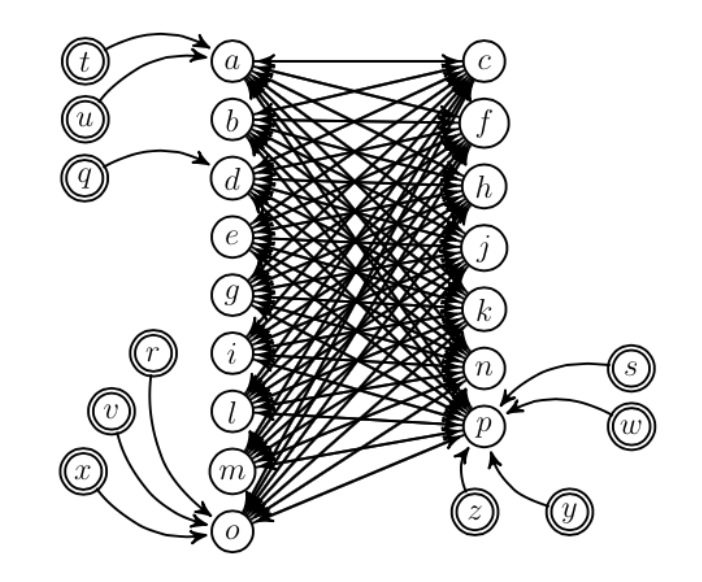
\includegraphics[width=0.5\textwidth]{argumentationframework}
\label{fig:argframework}
\end{figure}

Once arguments have been formulated in an AF it must be determined which arguments are admissible. Figure ~\ref{fig:arginteration} shows an typical interaction. Within an argumentation framework an argument A can become inadmissible if it is attacked by another argument B. However, if B is attacked by C and becomes in admissible then A may be reinstated.

\begin{figure}[!h]
\centering
\begin{tikzpicture}

\tikzset{vertex/.style = {shape=circle,draw,minimum size=1.5em}}
\tikzset{edge/.style = {->,> = latex'}}
% vertices

\node[vertex] (a) at  (0,0) {$a$};
\node[vertex] (b) at  (1.5,0) {$b$};
\node[vertex] (c) at  (3,0) {$c$};

%edges
\draw[edge] (c)  to[bend left] (b);
\draw[edge] (b)  to[bend right] (a);

\end{tikzpicture}
\caption{A is reinstated since C attacks B}
\label{fig:arginteration}
\end{figure}

As many arguments within an AF interact in this way, determining which arguments are admissible is difficult. Dungs solution is to use extension semantics to determine these arguments. These semantics contain conditions that a subset of arguments in an AF must satisfy in order to be collectively justified. Different semantics apply varying levels of strictness to the interpretation of what arguments are justified.

Semantics are based on a number of definitions given by Dung. A set of arguments is considered to be conflict free if no argument in the set attacks another argument in the set. A formal method to identify how conflicts are resolved is known as a semantic.(\cite{baroni2011introduction}) The literature defines two approaches to computing semantics: the labeling approach and the semantic approach. In a labeling approach arguments may be defined as \textit{out}(if they are attacked), \textit{in} (if they recieve no attacks or if the arguments attacking them are labeled out) or \textit{undecided} (if a resolution cannot be immediately found). In the extension based approach the strategy is to look at groups of arguments that can win the conflict as opposed to individual arguments in the labeling approach. An argument $A$ is acceptable with respect to the set $S$ if every argument that attacks $A$ is attacked by an argument in $S$. A set is considered admissible if every argument in it is acceptable with respect to the AF. From these definitions Dung defined the \textit{preferred extension} as the maximum admissible set of arguments in the AF. A \textit{stable extension} is defined as a conflict-free set of arguments that attacks every argument not in the set. The \textit{grounded extension} of an AF is the smallest complete extension that exists within the set of admissible arguments. Each of the semantics interprets the AF in a different way, the preferred extension is more inclusive while the grounded extension is more skeptical. 

\begin{figure}[!h]
\centering
\begin{tikzpicture}

\tikzset{vertex/.style = {shape=circle,draw,minimum size=1.5em}}
\tikzset{edge/.style = {->,> = latex'}}
% vertices

\node[vertex] (a) at  (0,0) {$a$};
\node[vertex] (b) at  (1.5,0) {$b$};
\node[vertex] (c) at  (3,0) {$c$};
\node[vertex] (d) at  (4,1) {$d$};
\node[vertex] (e) at  (4,-1) {$e$};

%edges
\draw[edge] (b)  to[bend left] (a);
\draw[edge] (a)  to[bend left] (b);
\draw[edge] (b)  to[bend left] (c);
\draw[edge] (c)  to[bend left] (d);
\draw[edge] (d)  to[bend left] (e);
\draw[edge] (e)  to[bend left] (c);

\end{tikzpicture}
\caption{An example AF taken from \cite{baroni2011introduction}}
\label{fig:arginterationBaroni}
\end{figure}

In figure~\ref{fig:arginterationBaroni} the grounded extension is empty. There are two preferred extensions the set $\{a\}$ and the set $\{b , d\}$. The stable extension is $\{b , d\}$.

The implementation of a system based on defeasible reasoning and argumentation theory is a central focus of this project. This section has briefly outlined DR and AT at a high level for the reader. For a more detailed background in AT the reader is referred to \cite{bench2007argumentation}.

\subsection{Argumentation Theory Implementations}
\label{sec:dr_implementations}

Implementations of argumentation theory based systems tend to fall into two broad categories. One branch takes advantage of the computational power of the techniques to solve problems in medicine, law and online behaviour. The other implementations focus on creating GUI tools in order to improve the reasoning process of their users.

Argument diagramming tools leverage visualisation techniques to aid users in reasoning about arguments. This has practical applications in several fields.

\cite{twardy2004argument} demonstrated the advantages of computer based Argument mapping systems in improving student critical thinking. Twardy measured improvement in student performance on the California Critical Thinking Skills Test across a semester. Students from an ``introduction to critical thinking'' class were divided into three groups, two groups recieving normal course tutorials, the third group using Reason!Able (argument mapping) software. Students who used argument mapping software scored results on average three times higher than their peers by the end of the semester. Twardy believes that the students' critical thinking improved by using the software as it allowed them to distinguish between reasons and supporting premises.

In the same domain, \cite{reed2001araucaria} designed Araucaria to make argument diagramming for undergraduates easier and also to support research activities. In addition, the authors developed AML (Argument Markup Language) an XML based syntax for describing the structure of arguments. They explain the strength of their software as it's platform independence (it was developed in Java) and it's interoperability with other tools. Araucaria represents arguments in a tree structure with the branches of this tree representing support relations. This is in contrast to Dung's argumentation framework which uses edges to represent attack relations.

\begin{figure}[!h]
\centering
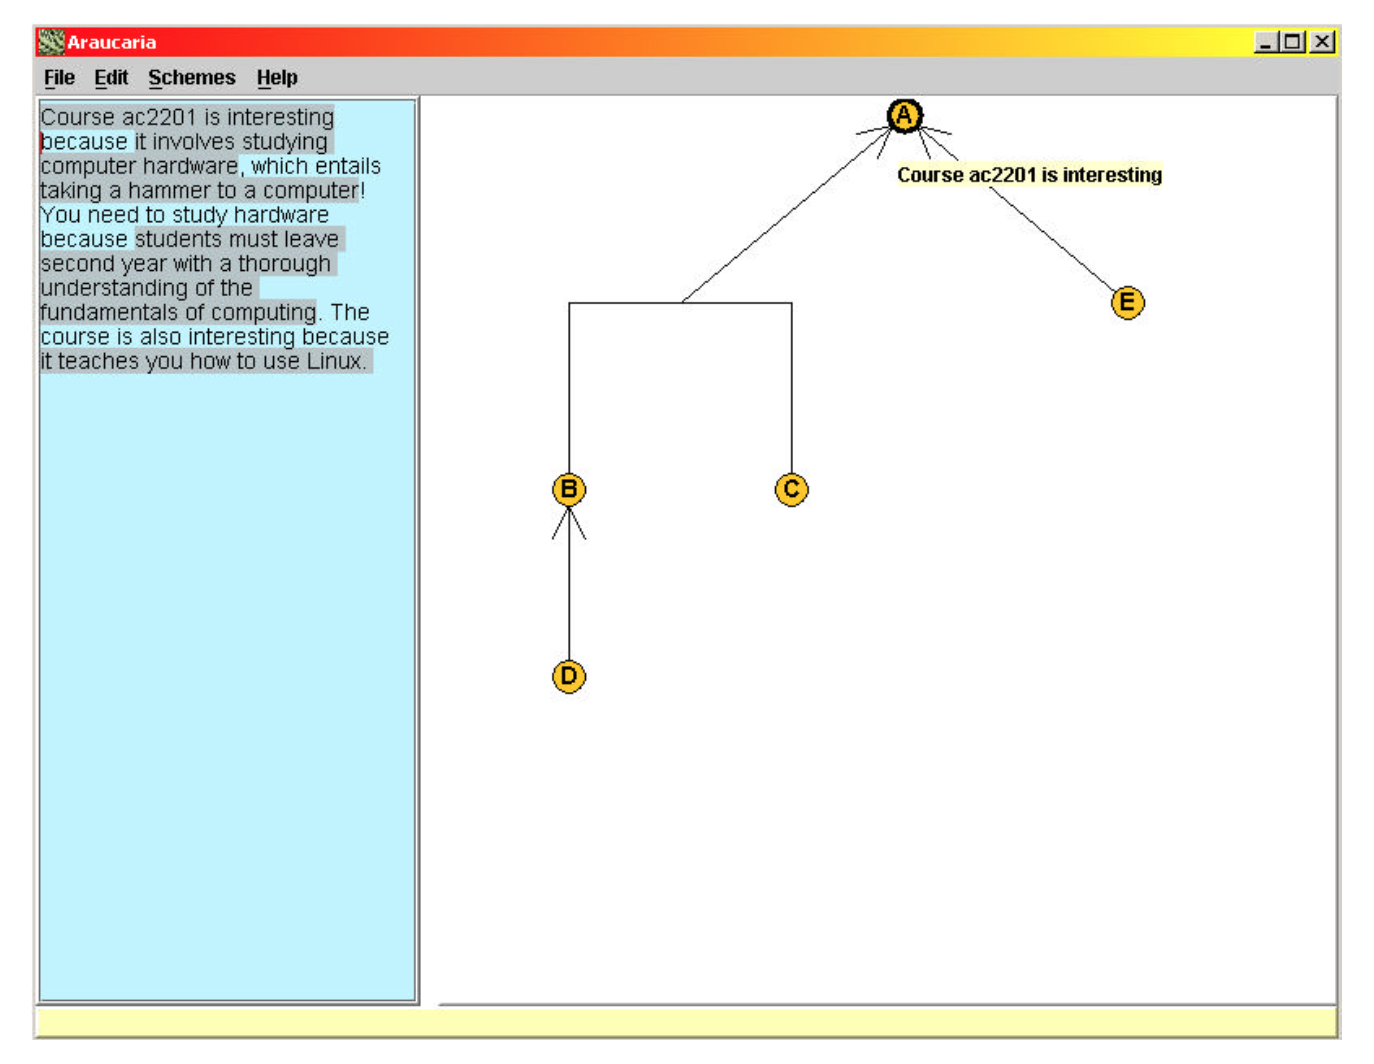
\includegraphics[width=140mm]{araucaria}
\caption{Argument diagramming with Araucaria}
\label{fig:my_label}
\end{figure}

\cite{karacapilidis2001computer} developed the HERMES system, an implementation of Argumentation Theory that allows users to collaboratively develop arguments online and support those arguments with data. HERMES also provides users with access to information from external databases to further justify their arguments. Arguments are represented using a labelling approach as opposed to a graph approach. Constraints are inserted into a discussion graph and when new constraints are introduced they are checked against existing ones.

The authors evaluated their system focusing on usability. A wide variety of users such as students, researchers and medical doctors were surveyed. The participants attempted to solve two problems collaboratively using the tool and then answered questions. These questions were both about the users overall opinion of the system (ease of use, enjoyable, intention to use again) and about effectiveness of the system (task clarity, easy to read, sufficiently informative). The tool focuses on collaborative decision making and not on automated output so there is no evaluation of task performance.

%this could be used for software evaluation
\cite{easterday2009design} surveyed many argument mapping tools, listed shortcomings common to the tools and developed requirements for argumentation tools from this list.
The six requirements listed are correct visual representation, flexible construction, control over visual properties, automation of non-semantic operations, multiple diagrams for comparison and cross platform compatibility. As none of the avaiable tools at the time satisfied all of these requirements, the authors developed a prototype, iLogos that would fulfill these requirements.

The fact that decision support systems allow users to aggregate evidence and make decisions based on that evidence lends makes them an obvious fit for medical practitioners. \cite{hunter2010argumentation} developed a framework for generating inference rules to argue for and against the benefits of medical treatments based on evidence. Their work highlights the benefits of argumentation systems in abstracting away the complicated nature of medical evidence into a form more manageable for practitioners.

A review of defeasible reasoning implementations by \cite{bryant2008review} highlight the need for well designed empirical evaluations of implementations and formal complexity analysis to justify the practical applicability of a reasoning engine. The paper also highlights the proprietary nature of successful argumentation theory based applications preventing researchers from peer reviewing the software.

\cite{dimopoulosfinding} provided one of the initial complexity analysis of the approach proposed by Dung. The authors found that while many believed that Dung's AF would simplify the implementation of non-monotonic logics, it turns out that the computational complexity of Dung's AF is greater than that of standard implementations of non-monotonic reasoning. The authors outline that in a particular worst case scenario, ``Autoepistemic Logic'' the computational complexity is two orders higher than in a standard implementation. In the discussion of their results the authors underline that for the computational complexity is only better in for sceptical reasoning and only in trivial cases that are almost equivalent to classical logic.

\cite{vreeswijk2006algorithm} opposed the authors approach of specifically targeting worst case scenarios. Vreeswijk takes a more pragmatic approach designing algorithms that produce grounded and admissible semantics for practical implementation in systems. The author presents average and best-case complexity as well as worst case complexity. He states that the admissible membership problem is NP-complete; for the worst case the complexity grows exponentially with the number of nodes. The algorithm developed by the author is an efficient and practical one and has been ultilised in serveral implementations of AFs including the Dung-o-matic used in this project.

\cite{modgil2014aspic+} presented a tutorial introduction to ASPIC+; a framework for specifying argumentation systems, rather than an implementation of a system. The authors claim that while Dungs calculus is indispensable, it provides little guidance for the development of a system based on his theories. ASPIC+ aims to provide guidance on how the constituent premises of an argument make up an attack. Within their framework arguments could be attacked in three ways: their uncertain premises, their defeasible inferences or on the conclusions of their defeasible inferences. They suggest their approach as a best practice for the development of argumentation systems.

\cite{egly2008aspartix} introduces Aspartix. Aspartix can compute the extensions that the authors consider to be most important from Dungs AF (admissible, prefered, stable, complete, and grounded). ASRARTIX uses answer set programming, a type of logic programming designed to solve intractable problems, in order to compute the semantics. The authors believe that implementing argumentation systems within this programming paradigm provides clarity not offered in other paradigms. It also offers a computational advantage since the computations that are intitially intractable may be reduced into another language which already has efficient solutions implemented in it. In order to run Aspartix a computer must already have an answer set programming solver like Gringo installed on the system. Users also interact with a web hosted version of Aspartix\footnote{\url{http://rull.dbai.tuwien.ac.at:8080/ASPARTIX/loadGraph.faces}}.

\begin{figure}
    \centering
        \subfigure[Input attacks and arguments]{\label{fig:a}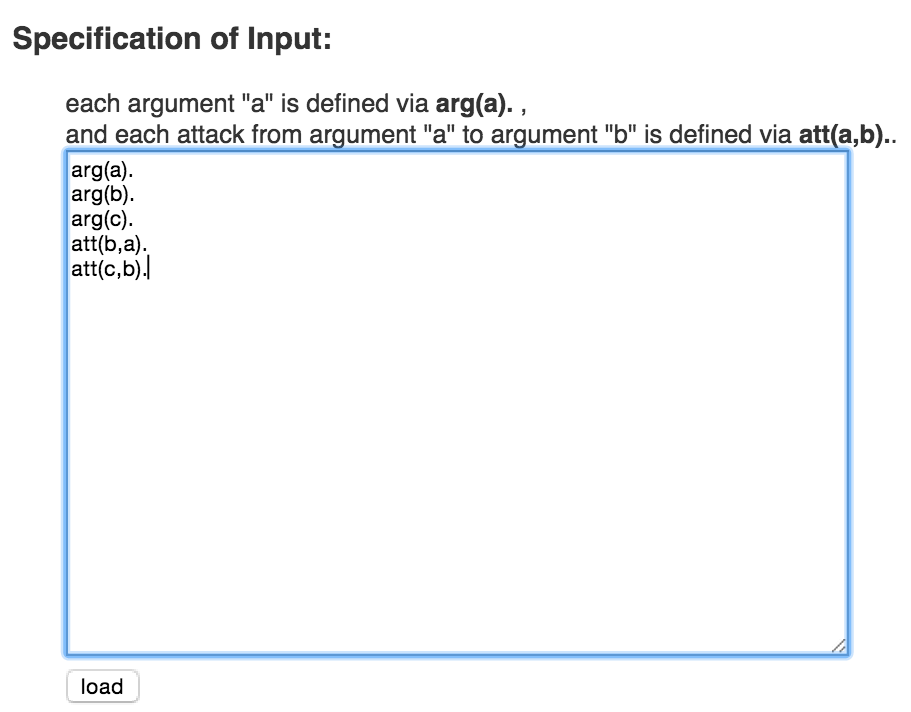
\includegraphics[width=70mm]{aspartixinput}}
        \subfigure[Output graph and semantics]{\label{fig:b}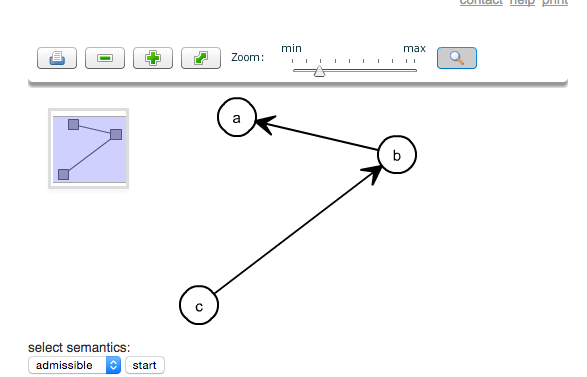
\includegraphics[width=70mm]{aspartixoutput}}
    \hfill
    \caption{The Aspartix web interface}
    \label{fig:three graphs}
\end{figure}

%argulab
Motivated by the desire to apply argumentation in multi-agent systems \cite{podlaszewski2011implementation} developed Argulab. Argulab is an attempt to provide a standard library of argumentation algorithms for use in multiple applications. The authors demonstrate the ability of Argulab to compute semantics, argument justification status, argument-based discussion and judgement aggregation.

Comparing the performance of programs to compute AF semantics is a challenging aspect of these new systems. \cite{cerutti2014generating} explains that the lack of a large set of challenging AFs makes benchmarking the algorithms difficult and offers a solution in the form of AFBenchGen.
AFBenchGen is a C++ program designed to generate random a AFs for benchmarking.
The program was able to efficiently generate large AFs with 5,000 nodes and 270,000 attacks. The authors explain that a more through test suite should contain AFs with different structures and determining how to generate these test cases is a subject for further study.

Two studies have built upon this work and benchmarked implementations designed to compute the semantics of Dung's AFs. \cite{bistarelli2014benchmarking} provide a performance comparison of the computation of stable semantics in ASPARTIX, dynPARTIX, Dung-O-Matic, and ConArg2. The semantics were benchmarked across three different graph structures; the Erdős-Re ́nyi model, the Kleinberg small-world model, and the scale-free Barabasi-Albert model. By focusing on stable semantics they focus on one of the worst case scenarios as a stable semantic doesn't always exist and it's computation is NP-Hard. Out of all four Dung-o-matic performed least favourably, ASPARTIX performed well at solving Erdos-Renyi but overall ConArg2 was found to be the strongest implementation.

\begin{figure}[!h]
\centering
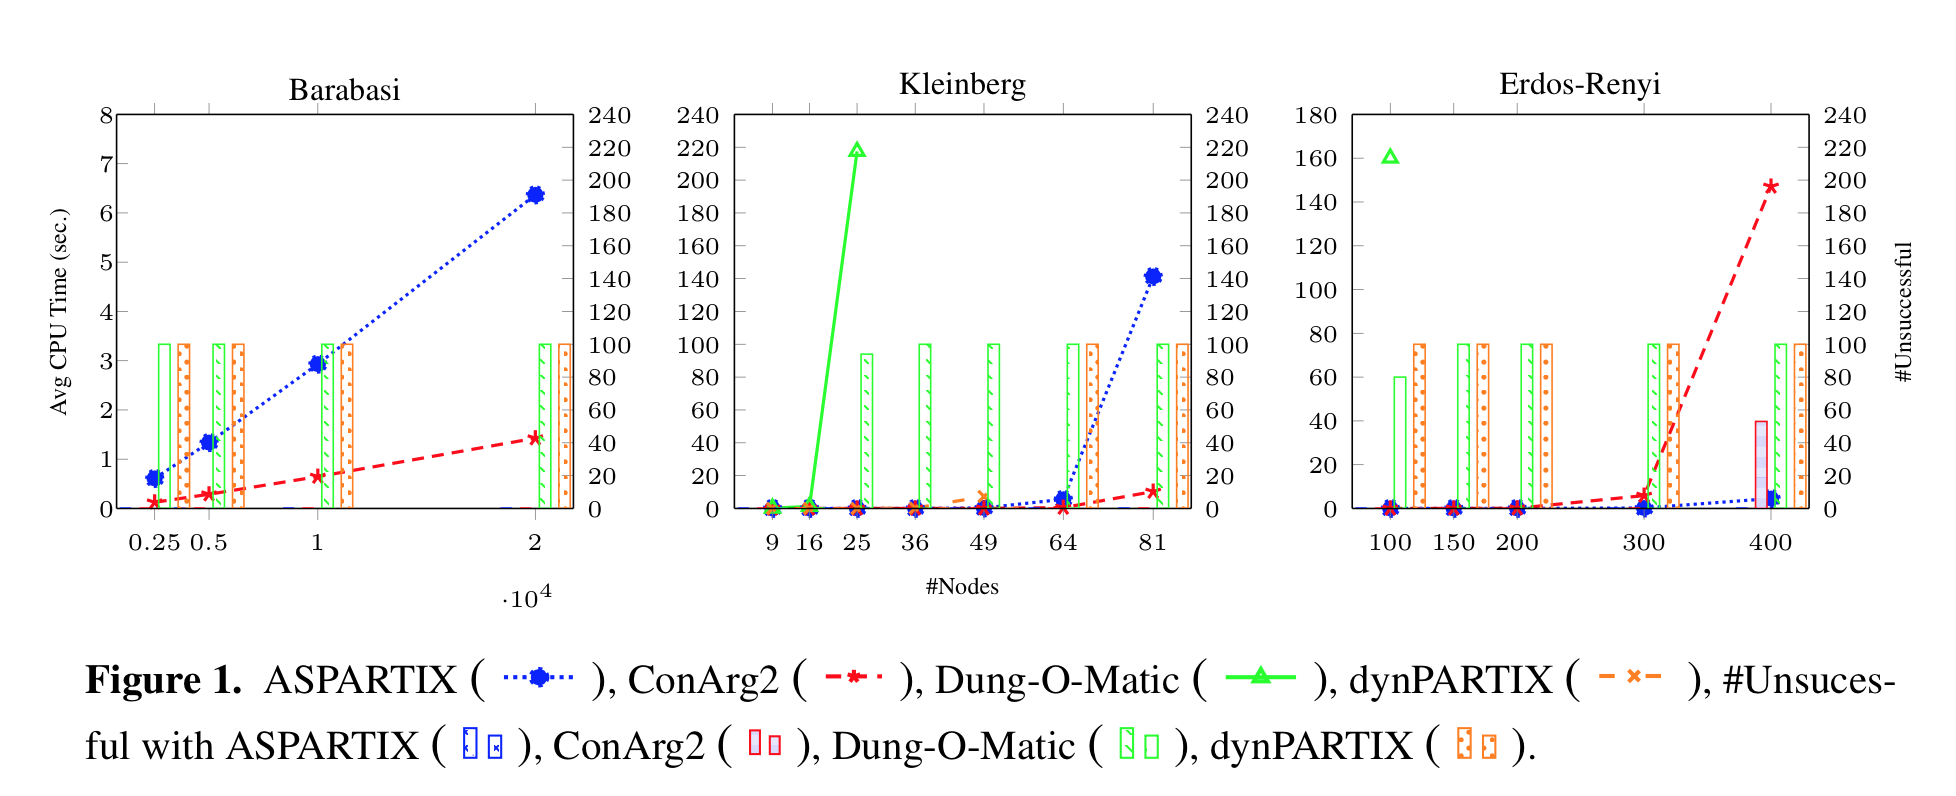
\includegraphics[width=140mm]{benchmark2}
\caption{Performance benchmarks taken from \cite{bistarelli2014benchmarking}}
\label{fig:my_label}
\end{figure}

These findings are echoed in earlier work carried out by \cite{bistarelli2013first} that found ASPARTIX and ConArg to significantly out perform Dung-o-matic. Similarly in this work the authors attempted to compute the complete and stable extensions for the three random graphs given above and also for Watts-Strogatz graphs. 

\begin{figure}[!h]
\centering
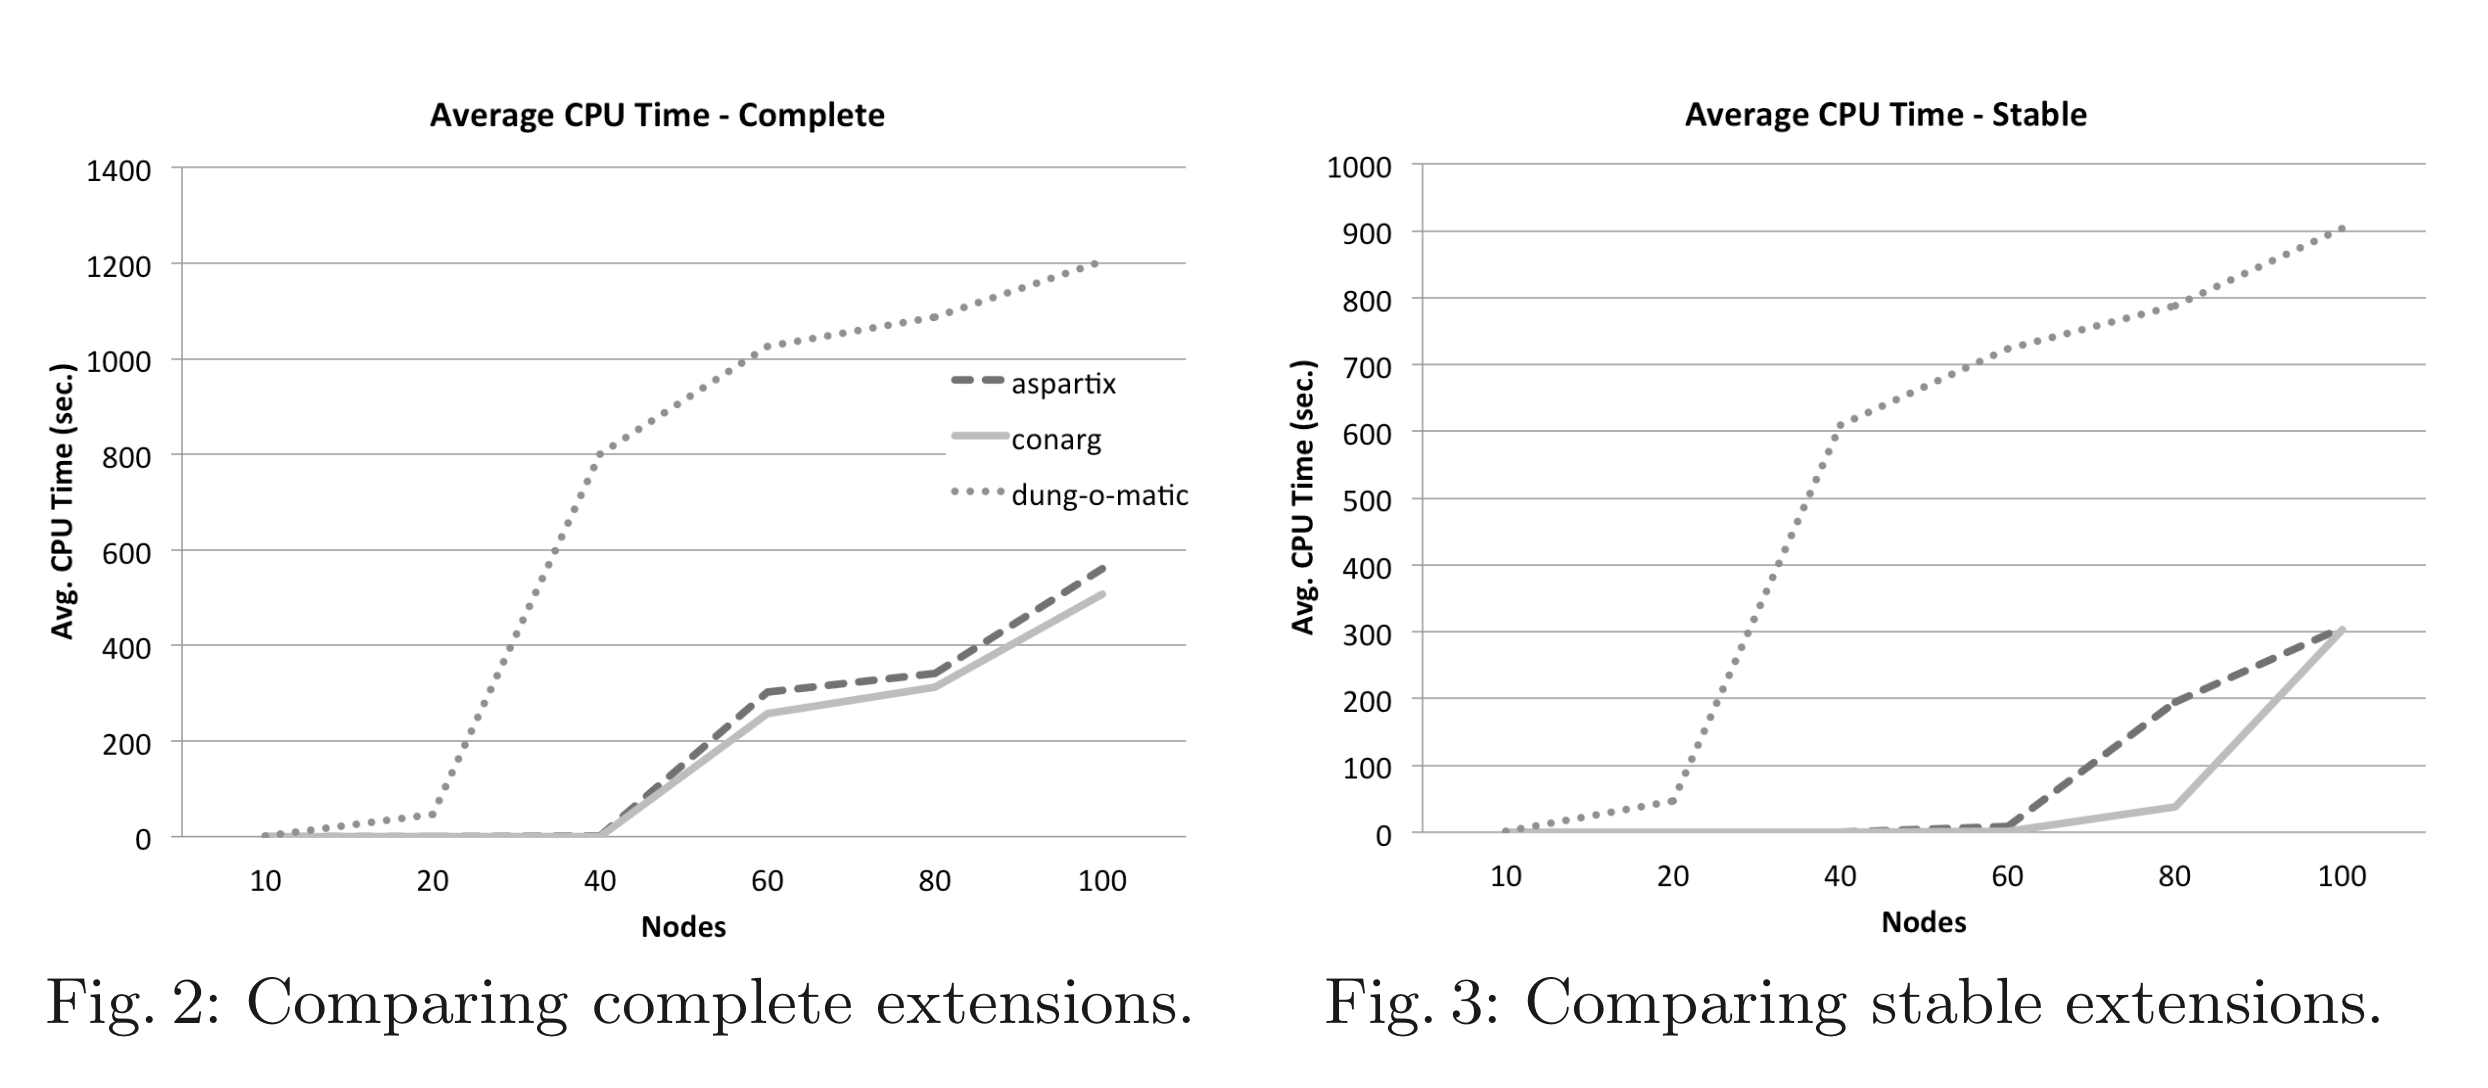
\includegraphics[width=140mm]{benchmarking}
\caption{Performance benchmarks taken from \cite{bistarelli2013first}}
\label{fig:my_label}
\end{figure}

An alternative to Dung's argumentation framework has been proposed by \cite{gordon2007carneades}. Their model contrasts with Dung's AF by considering the internal structure of arguments in evaluating their feasibility. The model uses directed graphs to model the argumentation process as well, however, there are additional elements instead of simply arguments and attack relations. Nodes may be arguments or supporting information such as datum, claim, warrant, backing and exception. The relationships between nodes may be attack or support relations and are distinguish by using different arrow heads. An implementation of their framework exists known as Carneades.

\begin{figure}[!h]
\centering
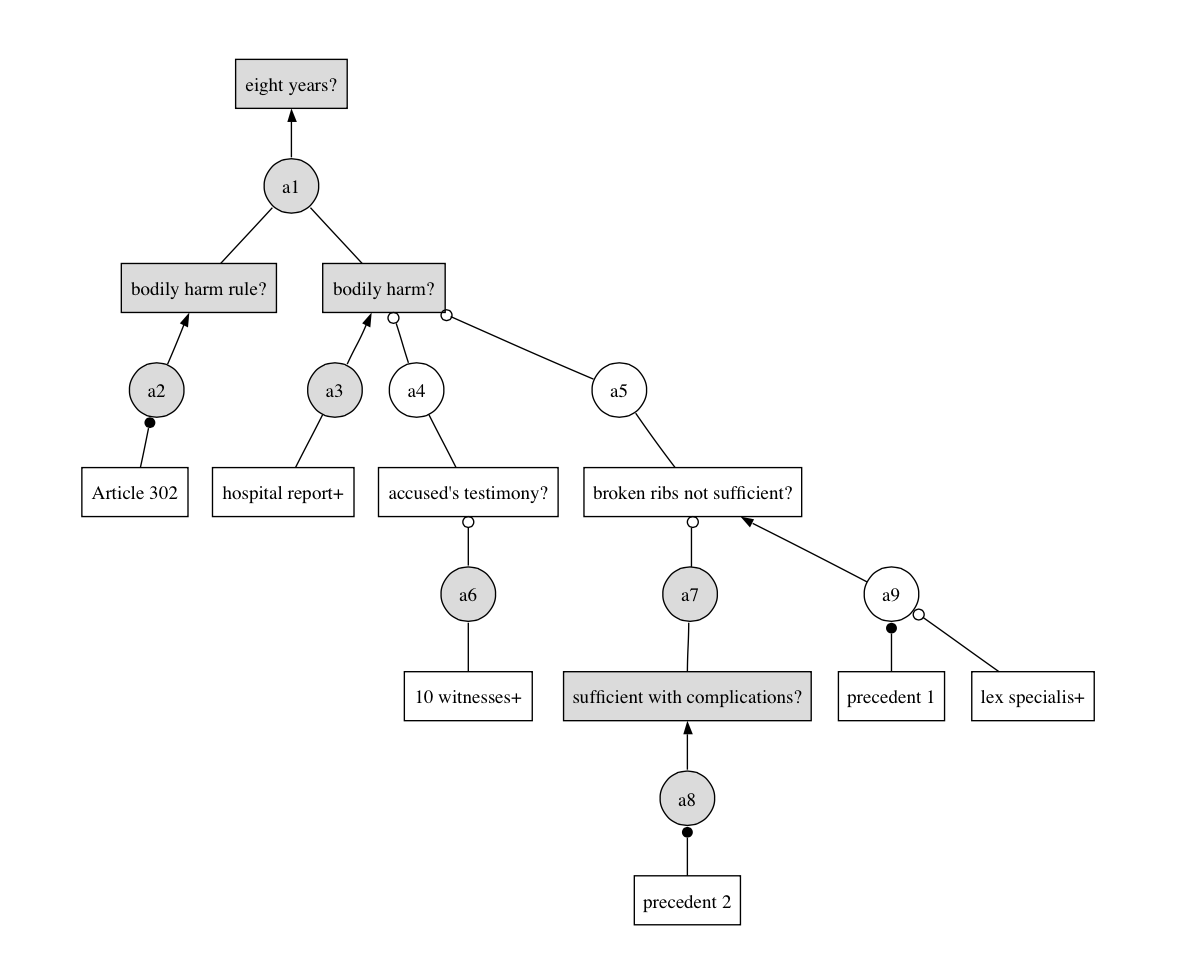
\includegraphics[width=140mm]{carnedes}
\caption{A Carnedes argument graph showing more complex relations than considered in a Dung-style AF}
\label{fig:my_label}
\end{figure}

\cite{van2014principled} provide techniques for translating Carneades argumentation frameworks into Dung style AFs in order to use the more efficient implementations.

While the Carnedes approach may be overly complex for practical purposes, it does underline the importance of considering the internal structure of arguments. Most of the implementations considered so far evaluate the semantics of an AF with respect to the framework as it is defined. However, whether arguments are relevant varies depending on the instance of data being considered.

% How do longo and hederman consider the activation of an argument
A comparison between argumentation theory and machine learning was made by \cite{longo2012argumentation} in the domain of health informatics. The comparison specifically tackled the ability of both approach to solve a classification problem; the recurrence of breast cancer. The authors developed a Dung style argumentation framework based on the knowledge base of a single health-care practitioner. The authors used this knowledge based to determine results for rows in a classic breast cancer data-set. In order to determine whether or not an argument in the framework was activated the authors used fuzzy membership functions. The authors then compared the results of this experiment with the predictive capacity of several machine learning algorithms (decision tables, bayesian networks, best-first and alternating decision tree, regression and multilayer perceptron) varying percentage of split and the number of folds. The results of their experiment showed that argumentation based systems could perform as well and in some cases better than machine learning algorithms. Moreover, as there was no training involved the approach was likely to perform equally well on a different data set, unlike the machine learning approaches.

Overall the advantages outlined by the authors highlight the `human' element of the approach. AT is more intuitive and can provide users with greater understand of the problems they seek to solve. Experts can subjectively compare knowledge bases and obtain explanations for results computed on the basis of their knowledge. The lack of the same human element in machine learning is what provides it's advantages over AT; training is automatic and doesn't require a knowledge base to be elicited. 


\section{Construct Modeling}

In order to answer the research question posed at the beginning of this dissertation the idea of a construct must be defined.
\cite{price2013research} discusses measurement in the context of psychology. He explains that many variables are simple to determine such as height, age, sex. We can gather this information by simply observing it. By contrast, a construct can be considered to be as a non-physical thing that cannot be simply measured.\footnote{For the purpose of this experiment, time is not a construct. Time can be measured with a watch.} 

Constructs are ideas people have about things, they may be idealised or may not really exist. Constructs are useful in science for improving our understanding of difference phenomena and techniques are often established in an attempt to quantify them. Examples of such constructs include intelligence (measured using IQ tests), personality (measured using surveys) and evolution (measured using changing characteristics over generations).

Representing constructs in a computable manner offers many potential benefits. By automating the representation of constructs we can free up the time of experts, for example, by automating diagnosis. We can reduce human error, for example in the case of reasoning. We can make predictions about certain situations and generally improve our understanding of phenomena. 

Developing systems that can represent constructs accurately is not trivial. There are a number of underlying issues that make solving this problem hard. Evaluating the performance of such systems is challenging as we have have no external measurement to compare the construct with. The same issues of implementation that occur in regular systems occur in these systems as well. There are a number of areas errors could arise:

\begin{itemize}

  \item Problems could occur as a result of errors in the data set
  \item the experts knowledge about the construct could be unsound
  \item the entire school of thought about the construct could be unsound
  \item the experts knowledge might be modeled incorrectly in the system
  \item the design of the system may be flawed drawing incorrect conclusions
  \item the implementation of the system may have underlying bugs that the software developer is unaware of.
  
\end{itemize}

In order to mitigate against these kinds of problems special care should be taken in gathering data for experiments. Experts should be selected carefully for modeling knowledge bases. There isn't much that the designer of a system can do to ensure that the knowledge of an entire field of study is correct. However, by interacting with a system for the evaluation of constructs, experts may gain a deeper understanding of the phenomena that they study. To ensure that an expert's knowledge base is modeled correctly user interfaces to the system should provide clear feedback and knowledge engineers should be trained to use them appropriately. Special care should be taken in the design of the system and appropriate test cases determined.

In order that a system can be evaluated using the techniques discussed in  section~\ref{sec:evaluation} the data set must contain some representation of the construct being studied. One method for evaluating the representation of the construct would be to have an expert manually determine labels for each row in a data set. These labels can then be compared with the output of an experiment to determine the accuracy of the output. 

This method is problematic as it is time consuming and may not yield accurate results. In order that a label is applied correctly an expert will need to study each row the data individually and take the time to assess it accurately. As this would need to be done for thousands of rows it will take up a lot of time. On top of this, the work is tedious so many experts will apply less scrutiny to each row resulting in less accurate labels.

Alternatively, the output can be compared with columns already present in the data but not used in the final result. It might be determined that there is a strong correlation between the construct and some other variable. If this variable is not included in the determination of the construct then we can measure the accuracy of our construct by seeing how it correlates to this variable.

Constructs are typically made up of interleaved ideas and variables which makes their representation in computer systems complex. The structure of constructs varies and as a result different models may be developed to measure them. Similarly, different computational techniques may be used to represent these models.

For example, if we take intelligence as a construct, there are a number of approaches we could use to measure it. Intelligence can be represented by IQ; by computing the sum of an individuals scores on questions across a number of domains. If intelligence is modeled in this manner then it is easy to derive the model using linear regression. If on the other hand a more complex scoring system was used then a different supervised machine learning technique could be used. Similarly an expert could communicate with a group of people in a room and give their opinion on which people they believe are intelligent. This opinion then be used as labels for a data set in which a (very bad) model of intelligence could be made by training a classifier based on age, weight, sex etc. In another case, we could run clustering algorithms on out data. If the algorithm returns two clusters and one cluster has all the Nobel prize winners we might conclude that is the intelligent cluster. An expert could model intelligence defeasibly. For example, if someone performs well on tests they are intelligent but if they cheat on tests they are not. We could run semantics on those defeasible representations to determine who is intelligent.

None of the approaches outlined above can objectively say that they truly measure intelligence. However, if they are useful they will give some indication of how a person will perform on a task. The purpose of this example is to underline the differences in models and how these models can be represented using computational techniques.

It is with this in mind that an experiment is designed to compare these techniques. To do an experiment this has to be done:

\begin{itemize}

  \item A suitable construct must be chosen and access to an expert secured.
  \item Machine learning software must be procured and a number of machine learning techniques chosen for evaluation.
  \item A system based on defeasible reasoning must be designed.
  \item an experiment built on top of this must be chosen 
  
\end{itemize}




\section{Evaluation of Knowledge-based Techniques}
\label{sec:evaluation}
As the overall aim of the research project is to compare an implementation of defeasible reasoning with machine learning, a framework for comparing the two must be developed. This is no easy task as the techniques vary considerably in the output they will produce. For supervised machine learning the output of the experiment will be a number or a classification. These numbers and classes will already be present in the training and test data sets. For defeasible reasoning this is not the case. The implementation outputs a value that is a representation of a construct. In the experiments performed for this project, that construct is mental workload. There are many ways to measure mental workload but there is no one definitive value that can be used for comparison with this value. There is no value already present in the dataset that we can compare the output of the defeasible reasoning system with.

The following section gives an overview of the various methods used to evaluate the techniques in work by previous authors.



\subsection{Construct Validity}

As the aim of this project is to compare the ability of machine learning and argumentation theory to represent and predict the value of a construct, an investigation into construct validity is necessary. Constructs can be thought of as things that are not easy to observe. The are difficult to measure as they are often ambiguous, abstract and can be quite complex. Measuring constructs requires that they are defined precisely and a way to translate the construct from the abstract to the concrete is established.

Construct validity refers to the accuracy of this translation. Construct validity is not refered to in absolute terms, however, we can say that over time a certain measure has shown strong construct validity\footnote{See \url{http://dissertation.laerd.com/construct-validity.php}}. Two measures used to determine construct validity are concurrent validity and convergent validity.

Concurrent validity is used to establish that a particular measure may be used to predict some other outcome that is determined by the construct. The outcome to be verified against must be collected in the same experiment as the new measure being explored.\footnote{\url{https://explorable.com/concurrent-validity}} The ability of the new contruct to predict this outcome can then be determined by using a regression model. A notable flaw in concurrent validity is that the measure used to benchmark the new measure may itself be flawed. As a result of this it is rarely used alone but has been used with other measures to assess the validity of a wide variety of constructs such as social anxiety by \cite{la1993social}, martial satisfaction by \cite{schumm1986concurrent} and depression by \cite{storch2004factor}.

Another means of determining the validity of a measure is the convergent validity of a measure. Concurrent validity was introduced by \cite{campbell1959convergent}. If there already exists some accurate measure for the construct that is being examined, the new measure can be evaluated by looking at it's relationship to the old measure (how the two converge). Convergent validity can be established by computing a correlation between the new measure and an old measure. This suffers from the same problems as concurrent validity since the measure used as a benchmark may be flawed. Convergent validity has also been widely used, for example in establishing measures for post traumatic stress disorder (\cite{neal1994convergent}), social desirability (\cite{stober2001social}) and social phobia(\cite{beidel1996assessment}).

\subsection{Diagnosticity}

%-----------------------------------
%	MACHINE LEARNING
%-----------------------------------
\section{Learning Based Approaches}

The literature makes the distinction between different learning scenarios: supervised and unsupervised. 

\section{Supervised Machine Learning}
\cite{alpaydinintroduction} explains that `supervised learning' happens in a scenario in which the task of the algorithm is to learn the mapping from some input X to an output Y. In a review of supervised learning classification techniques, \cite{kotsiantis2007supervised} explains that if ``known labels (the corresponding correct outputs)" are used ``then the learning is called supervised". Examples \footnote{Taken from Kaggle.com; a website for data science competitions} of questions supervised learning attempts to answer include:

\begin{itemize}
  \item What is the probabilistic distribution of hourly rain given polarimetric radar measurements?
  \item What category does a particular product belong to given it's features?
  \item Given a number of objective measurements, what will be a restaurant's annual sales? 
\end{itemize}

Supervised learning problems can be further divided into two categories; regression problems and classification problems. 
\cite{ng2000cs229} explains that regression problems are problems where the output to be predicted is continuous. In a regression problem as specific numeric value is predicted, for example, a restaurant's annual sales in the example above. Problems in which the output to be predicted is discrete are considered classification problems. Classification problems tend to be concerned with the sorting of data into correct categories, as in the second example above. Another such problem might be determining whether or not a particular email should be categorised as spam or not.  

The following sections introduce the reader to supervised machine learning techniques relevant to this project from each of the different categories at a high level. Many of the techniques outlined require a strong understanding of mathematics in order to fully understand and engage with them. This outline will avoid these details as explaining them sufficiently is beyond the scope of this project.

% naivebayes
\subsection{Naive-Bayes}
\cite{kohavi1997improving} introduces Naive-Bayes or Simple-Bayesian Classifier and then outlines techniques for it's improvement. The learner is ``built based on a conditional independence model of each attribute given the class.'' Put simply the learner uses probability to classify the data. Bayes refers to Bayes rule, a mathematical rule for computing the probability that something happens given some other \textit{a priori} condition. The technique is called Naive as the probabilities of the features in the model are assumed to be independent. The probability of each class is computed for a row in the data set. The class with the highest probability for that row is the class that is chosen for that instance of the data.

\subsection{Bayesian Networks}

\cite{export:69588} explains that Bayesian Networks have been increasingly employed in expert systems as an encoding for an experts knowledge. One of the strengths of Bayesian Networks is that they can still produce an output with incomplete data. Bayesian Networks provide methods for dealing with uncertainty by graphically modelling dependent relationships. Each attribute is modelled as a vertex in the graph with the relationships modeled as edges. Internally the nodes have a table containing the probability outcomes given conditions have occurred in their parent nodes. In figure~\ref{fig:bayesnet}, an example taken from \cite{witten2005data} the probability of the temperature being hot, mild or cool depends on the values of play and outlook. The table appears as in table~\ref{tab:bayes_table}.

\begin{figure}[h]
\centering
\begin{tikzpicture}

\tikzset{vertex/.style = {shape=circle,draw,minimum size=1.5em}}
\tikzset{edge/.style = {->,> = latex'}}
% vertices

\node[vertex] (a) at  (3,0) {$play$};
\node[vertex] (b) at  (3,2) {$humidity$};
\node[vertex] (c) at  (2,4) {$temperature$};
\node[vertex] (d) at  (0,2) {$outlook$};
\node[vertex] (e) at  (0,0) {$windy$};

%edges

\draw[edge] (a) to (b);
\draw[edge] (a) to (c);
\draw[edge] (a) to (d);
\draw[edge] (a) to (e);
\draw[edge] (c) to (b);
\draw[edge] (d) to (c);
\draw[edge] (d) to (e);

\end{tikzpicture}
\caption{An example of a Bayesian Network from \cite{witten2005data}}
\label{fig:bayesnet}
\end{figure}

\begin{table}[h]
\centering
\begin{tabular}{|ll|lll|}
\hline
 play & outlook & hot & mild & cool \\ \cline{1-5} 
 yes & sunny & 0.413 & 0.429 & 0.429 \\ 
 yes & overcast & 0.455 & 0.273 & 0.273 \\ 
 yes & rainy & 0.111 & 0.556 & 0.333 \\ 
 no & sunny & 0.556 & 0.333 & 0.111 \\ 
 no & overcast & 0.333 & 0.333 & 0.333 \\ 
 no & rainy & 0.143 & 0.429 & 0.429 \\ 
\hline
\end{tabular}
\caption{The table of probabilities associated with the temperature node in figure~\ref{fig:test} }
\label{tab:bayes_table}
\end{table}

While Bayesian Networks are typically developed by mathematicians they can also be learned using ML techniques. 


% decisiontable
\subsection{Decision Tables}

\cite{kohavi1995power} proposed decisions tables as a representation for hypothesis in order to solve supervised machine learning problems. Decision tables are typically used in the development of rules in expert systems. The table consists of a list of conditions and actions to be taken depending on what conditions are met. An example decision table taken from \cite{hoffer1999modern} is given in figure ~\ref{fig:decision_table}.

\begin{figure}[!h]
\centering
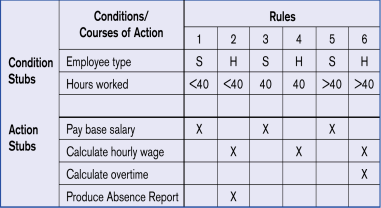
\includegraphics{decision_table}
\caption{Decision table example taken from \cite{hoffer1999modern}}
\label{fig:decision_table}
\end{figure}

\cite{kohavi1995power}'s supervised technique uses an induction algorithm to develop a decision table who's default is the majority class in the data set (the decision table majority). The induction algorithm build a decision table based on training data. When the model is presented with a new instance of test data it checks the decision table for matches. If there are no matches it returns the majority class of the training data. If there are several matches with different classes the class that makes up the majority of the classes is chosen. Through experimentation the author determined that the technique performed with prediction accuracy comparable with C4.5, a decision tree algorithm.

\subsection{K Star}

\cite{cleary1995k} describes K*, an instance based learner that uses entropy as a distance measure. An instance based learner classifies an instance based on a database of labeled examples. K* uses entropy in order to determine which instance in the database the current instance is most like. The entropy can be determined by taking the Kolmogorov distance (the length of the shortest string) between the two instances. The author reports that through experimental validation K8 performed better than another instance based learner, the 1R algorithm.

\subsection{Linear Regression}

Simple linear regression is a fundamental technique in supervised learning used to solve regression problems. In simple linear regression the technique takes a data set with one explanatory variable and one dependent variable and attempts to fit a simple line to it. According to \cite{ng2000cs229} this line can be defined as $h_{\theta}(x) = \theta_0 + \theta_1 x$. The parameters $\theta$ that define the function are tweaked in order to minimise a cost function. An efficient way to do this is using a technique known as gradient descent.

Linear regression can be used with many explanatory variables; in this case it is known as multivariate linear regression. The same basic principles that apply to simple linear regression apply here but the function we are trying to optimise is  $h_{\theta}(x) = \theta_0 + \theta_1 x_1 + \theta_2 x_2 + \ldots + \theta_n x_n$. In order to compute the large number of multiplications that need to occur the calculations are often formulated as linear algebra problems. The advantage of formulating these learning algorithms as linear algebra problems is that many programming languages contain libraries with optimised methods for computing matrix operations.

\subsection{Logistic Regression}

The regression techniques described above can be slightly modified to classify labeled instances of a data set. \cite{ng2000cs229} gives the example of classifying an email as spam (assigned the value 1) or not spam (assigned the value 0). In this case logistic regression computes the probability that an email is spam. This probability is given by the hypothesis function:
$$h_\theta(x) = \frac{1}{1 + e^{-x\theta^T}}$$

If there are multiple labels that need to be accounted for in the data set then logistic regression can be still be used in a `one-vs-all' fashion. Each label has it's own unique hypothesis function that can be used to determine whether or not to apply that label to the data.

\subsection{Artificial Neural Networks}

\cite{shiffman2012nature} provides an introduction to Neural Networks. Neural networks attempt to model the way learning occurs in the brain by simulating neurons and axions. The fundamental unit of a neural network is a perceptron; similar to one neuron. A single perceptron takes a number of weighted input values, computes their sum and applies a sigmoid function (in a similar manner to logistic regression) to the sum. It then compares this to a label and computes the error. This error value is used to adjust the weights of the input values; this feedback process is how the perceptron `learns'. 

A single perception can only compute linearly separable hypotheses. In order to compute more complex hypotheses the perceptrons are linked in what is called a muli-layer perceptron. In a multilayer perceptron an input layer of perceptrons take the inputs and then passes their output to another `hidden' layer of perceptrons. There may be multiple hidden layers that the output propagates through until it eventually reaches the output layer. The error for the network is then computed and applied to the weights of each perceptron using a technique known as back-propagation.

\begin{figure}[!h]
\centering
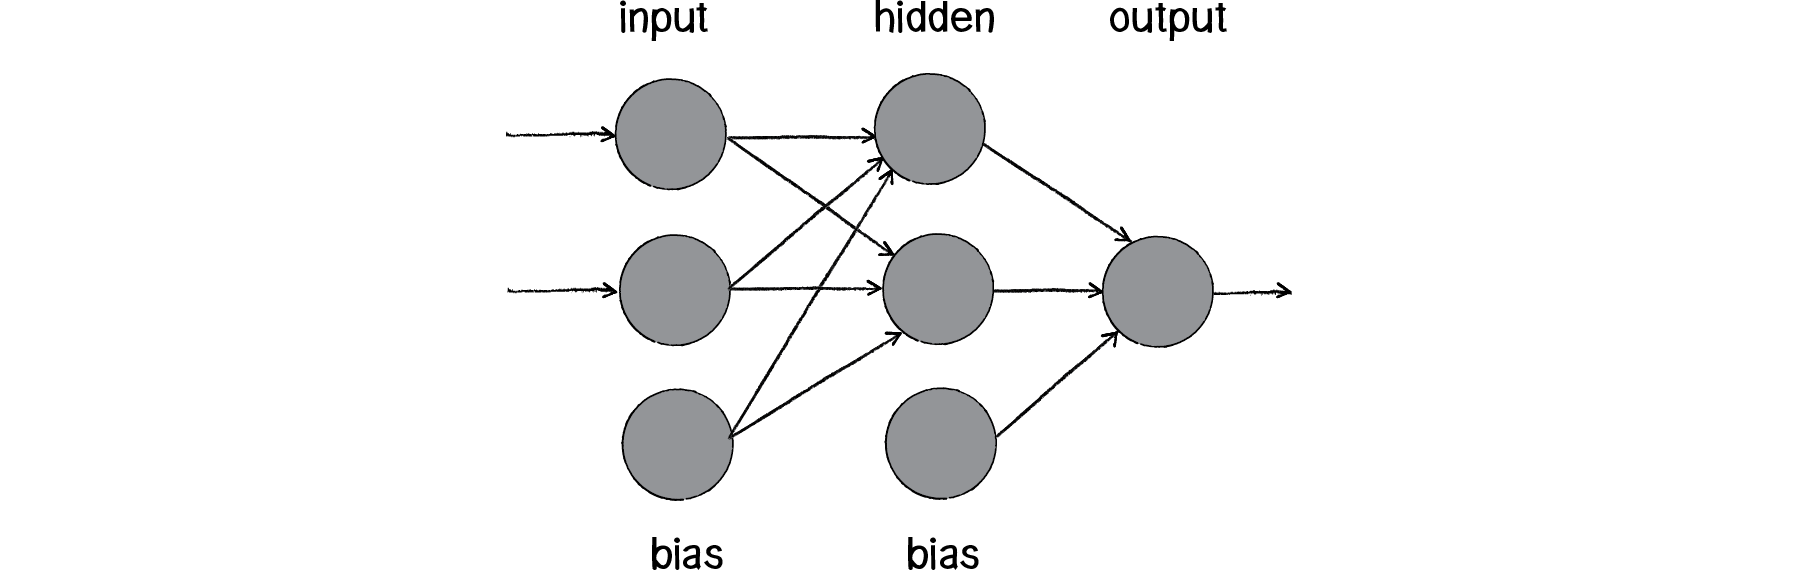
\includegraphics{multilayer}
\caption{An example of a multilayer perceptron taken from \cite{shiffman2012nature}}
\label{fig:my_label}
\end{figure}

The state of the art in machine learning is “deep” learning, currently being utilised by Google, Microsoft, IBM and others. \cite{arel2010deep} outline how deep learning overcomes the exponential growth in learning complexity associated with an increase in data dimensionality. Deep learning focuses on the development of computational models that represent information in a fashion similar to the neocortex. Convolutional Neural Networks are described as being the first successful approach to learning many dimensions in a complex manner. Deep belief networks are “probabilistic generative models”; provide a different solution to the problem of deep learning by providing probabilities associated with observations and labels bidirectionally.

\section{Unsupervised Machine Learning}

Supervised learning can be contrasted with unsupervised learning; described by \cite{mohri2012foundations} as problems in which ``the learner receives unlabelled training data and makes predictions for all unseen points.'' The learning is called unsupervised because the techniques don't attempt to make predictions based on a specific labeled output. Instead unsupervised learning techniques are used to perform tasks such as identifying clusters in data, anomaly detection and dimensionality reduction. Examples of practical applications of unsupervised learning (taken from \cite{ng2000cs229}) are:

\begin{itemize}
  \item Organizing computer clusters.
  \item Social network analysis.
  \item Identification of market segments.
\end{itemize}

A commonly used unsupervised learning technique is K-Means.

\section{Evaluation of Machine Learning Techniques}

There are a number of methods typically used for evaluation of machine learning techniques. Numeric predictions are evaluated similarly to many scientific experiments using statistical values such as correlation and mean absolute error. Machine learning techniques for solving classification problems are often more detailed as the costs of false positives and false negatives may be different depending on the problem. Take for example the prediction of cancer recurrence. A false positive (that it is predicted cancer will recur when it will not) will result in a patient being examined by a doctor; on the other hand a false negative would result in the missed opportunity of early diagnosis, potentially costing a life.

\cite{witten2005data} explain that machine learning techniques are typically evaluated first developing a model using a labeled `training set' of data. Once the model has been developed it can be run on a labeled `test set' of data. The performance of the technique can then be measured by comparing the values predicted by the model with the labels in the test set. The exception to this is with unsupervised machine learning as the data is unlabeled. As the purpose of unsupervised machine learning is to come up with a kind of `theory' about the data, good techniques ``make everything as simple as possible, but not simpler''. This idea is the foundation of the Minimum Discription Length Principle.

Typically the amount of data used for training and testing is limited and so techniques such as cross validation and percentage of split may be used to test and validate the model. In percentage of split the data set is divided into two groups, one for training and one for testing. Typically a higher percentage is used for training the data than testing it. In cross validation a data set is divided into groups. One group is used at a time for testing the model while the rest of the data in the set is used for training it. This technique is often referred to as N-fold cross validation where N is the number of groups the data is divided into. 

The following is a brief description of a number of measures used when evaluating the results of machine learning techniques.

\subsection{Numeric Prediction Problems}

\cite{witten2005data} explain that for practical situations the best numeric prediction method tends to perform well across all performance measures. Most performance measures tend to give an overall value for the difference between the predicted and actual value in a test set. Examples of such measure include mean-squared error, root mean-squared error and mean absolute error. As mean squared error squares the difference from the mean it tends to punish large errors more than the other measures.

Mean-squared error can be defined:

$$\frac{\sum \limits_{i=1}^n (p_{i} - a_{i})^2}{n}$$

Where $p$ are the predicted values and $a$ are the actual values.

Another performance measure used for numeric prediction problems is Pearson's Correlation Coefficient. This measures the linear correlation between the predicted value and the actual value. It differs from the other measure in that it ignores the differences in the scale of the two values.

$$\frac{S_{PA}}{\sqrt{S_{P}S_{A}}}$$

where:

$$S_{PA} = \frac{\sum _{i}(p_i - \bar{p})(a_i - \bar{a})}{n - 1}$$

$$S_{P} = \frac{\sum _{i}(p_i - \bar{p})^2}{n - 1}$$
$$S_{A} = \frac{\sum _{i}(a_i - \bar{a})^2}{n - 1}$$

\subsection{Classification Problems}

\subsection{Minimum Description Length}

\cite{grunwald2005tutorial} gives an overview of how the Minimum Description Length Principal is used to solve the problem of model selection. Overfitting is a problem that occurs frequently with ML techniques. Overfitting occurs when a learning technique puts too much emphasis on fitting the data exactly. As a result data points like outliers can skew the model and result in it classifying future instances of the data wrongly. A model that overfits the data will classify the data set used to train it with very little error, however, when used on a test set will perform poorly. A simpler model may not classify the training data perfectly but will perform better on test data.

As observed earlier, a simpler theory is one that allows data to be encoded using fewer bits. This idea is born from information theory. For example, the SVG file type encodes a red circle as \lstinline{<circle cx="50" cy="50" r="40" stroke="black" stroke-width="3" fill="red" />}. This is far simpler than sending every single bit used to describe circle in raw data. From the perspective of programming MDL can be compared to Kolmogorov Complexity; the simplest theory is the one that produces the shortest computer program that will print the data.

MDL views learning as data compression; \cite{grunwald2005tutorial} defines this formally: ``for a given set of hypotheses H and data set D, we should try to find the hypothesis or combination of hypotheses in H that compresses D most.'' The best point hypothesis H to explain the data D is the one which minimizes the sum L(H) + L(D|H), where
\begin{itemize}
  \item L(H) is the length, in bits, of the description of the hypothesis; and
  \item L(D|H) is the length, in bits, of the description of the data when encoded
\end{itemize}
with the help of the hypothesis.

The underlying idea of that can be derived from the principle is that the simple representation of constructs should be considered favourable to one that is complex. An informal approach to computing the MDL of a model is to describe a model in terms of the number of lines of code it would take to output the data. The greater the number of lines of code, the greater the MDL.

\section{Conclusions}

This chapter began with an exploration of two broad domains; machine learning and knowledge base systems. Within machine learning several supervised learning techniques were explored; bayesian networks, naive bayes, artificial neural networks, kstar and various regression techniques. Knowledge based techniques were explored and in particular argumentation theory and defeasible reasoning were introduced. In particular the fundamental work of \cite{dung1995acceptability} was introduced. This lays the foundation for the defeasible reasoning implementation of this experiment. Implementations for the computation of AF semantics have been reviewed in order to be integrated in this design. The results of other work using argumentation theory have been explored. 

Argumentation theory is advantageous as it allows for default reasoning but also to come up with solutions in the case of conflicting data. Linear regression is intuitive for developers and researchers as fitting a line to data is a familiar task. Linear regression is like default reasoning in that the line attempts to model things that happen typically. Outliers can be ignored as deviations from the norm and good predictions can be made most of the time. Linear regression considers outliers to be noise in the data and attempting to accommodate these outliers results in a model that overfits the training data. With a reasoning based approach data can be evaluated with greater scrutiny that can't be captured automatically through learning. Experts can provide the insight into why a particular outcome occurred, this could be modeled defeasibly in a way that wouldn't be captured by simply plugging data into an equation. A more complex machine learning technique such as an ANN could account for an outlier in a process like reasoning, however, it would need to be provided with data with enough instances of similar outliers that is similarly labeled. A data set large enough to train a classifier sufficiently to accommodate for these outliers may not exist. One this hypothetical classifier has been trained the resulting representation is possibly not ready to be interpreted by an expert. The automatic nature of machine learning has advantages that could not be obtained using a knowledge based approach. For example it would be difficult and time consuming for an expert to codify all of the different ways a person might write the letter `t'. An artificial neural network can be trained to recognise the letter if provided with enough labeled training data.

Both knowledge based approaches and learning based approaches fall in the field of artificial intelligence. Despite this there are relatively few works that provide comparison between the two. Within each approach exist many variations in techniques and algorithms with more being created as years go by. To specialise in one domain takes researchers years of focus; many would rather focus on advancing their research further than taking a step back to look at what research has been done in other fields. This is reasonable as it can take months of study to become familiar with even the basic concepts in an entirely different domain. A comparison made at this stage would likely be biased and would fail to account for the subtleties of one approach or another. Researchers that investigate both fields tend to do so to create advanced hybrid approaches (for example \cite{gomez2004hybrid}) rather than provide a comparison for the benefit of the research community. This research project attempts to fill that gap by providing such a comparison. The comparison of the two domains is a non-trivial task and it is unreasonable to expect it to be without bias. This project will attempt to provide some value to readers interested in both domains, however, it is to be considered by no means exhaustive.

A number of argumentation theory implementations were surveyed. Many of these implementation focused on aiding users in their reasoning. This focus has likely come about because it is a domain in which argumentation theory has an obvious immediate application. Graphical tools that incorporate the argument diagramming and the computation of results are less likely to be developed as they require several design issues to be resolved such as argument activation by data. It is also difficult for designers to know before implementation that such a system will fulfill a practical purpose.

Several techniques for assessing the predictive capacity of the techniques have been identified. Measures for establishing the validity of the construct measures have been determined. These measures will be valuable when assessing the techniques in a quantitative experiment as they will provide some objective way to compare results. None of these measures are perfect. Error values obtained during experiments of this nature may be misleading as the data used to train classifiers comes from the same set of data that is used to validate those classifiers. The measures being used to validate the representation of constructs are similarly imperfect. These measures rely on a correlation between the new measure and a previously established measure of the construct. If the previously established measure in fact is a poor representation of the construct then we may have simply created another poor representation. These factors will need to be considered in order to thoroughly evaluate the results of the experiment.